% =====================================================================
%  IT4868 - Web Mining - Project Report
%  Compiles with pdfLaTeX or XeLaTeX (Vietnamese names need the T5
%  font encoding or fontspec; both are set up below).
%  Upload figures/ together with this file. Charts are drawn by
%  figures/make_figures.py from the tables in data/report.
% =====================================================================
\documentclass[12pt,a4paper]{report}

\usepackage{amsmath,amssymb}
\usepackage{iftex}
% TeX Gyre Termes (Times-like, ships with TeX Live, covers Vietnamese).
% Works with pdfLaTeX (T5 encoding) and with XeLaTeX / LuaLaTeX (fontspec).
\ifPDFTeX
  \usepackage[utf8]{inputenc}
  \usepackage[T1,T5]{fontenc}
  \usepackage{tgtermes}
\else
  \usepackage{fontspec}
  \setmainfont{texgyretermes}[Extension=.otf, UprightFont=*-regular,
    BoldFont=*-bold, ItalicFont=*-italic, BoldItalicFont=*-bolditalic]
\fi
\usepackage[a4paper,left=2cm,right=2cm,top=3.8cm,bottom=2.2cm,
  headheight=50pt,headsep=20pt,footskip=1cm]{geometry}
\usepackage{fancyhdr}
\usepackage{booktabs,tabularx,array,multirow}
\usepackage{enumitem}
\usepackage{xcolor}
\usepackage{graphicx}
\usepackage{tikz}
\usetikzlibrary{positioning,arrows.meta}
\usepackage{caption}
\usepackage{float}
\usepackage[hidelinks]{hyperref}
\usepackage{titlesec}

\setlist{itemsep=2pt,topsep=3pt}
\setlength{\parindent}{0pt}
\setlength{\parskip}{5pt plus 1pt}
\captionsetup{font=small,labelfont=bf,skip=4pt}
\titlespacing*{\paragraph}{0pt}{4pt}{0.6em}
\emergencystretch=3em
\newcolumntype{Y}{>{\raggedright\arraybackslash}X}
\titleformat{\chapter}[hang]{\Large\bfseries}{CHAPTER \thechapter.}{0.6em}{\MakeUppercase}
\titlespacing*{\chapter}{0pt}{0pt}{18pt}
\titleformat{name=\chapter,numberless}[block]{\Large\bfseries\filcenter}{}{0pt}{\MakeUppercase}
\renewcommand{\contentsname}{Table of Contents}
\graphicspath{{figures/}}

% ---- Header on every page after the cover (logo left, course info right, grey rule)
\newcommand{\coursename}{Web Mining - IT4868E}
\newcommand{\semester}{Semester 2026.1}
\newcommand{\reportheader}{%
  \fancyhf{}%
  % logo sits on the baseline (no part below it), so the rule cannot touch it
  \fancyhead[L]{
\includegraphics[height=1.45cm]{soict_logo.png}}%
  \fancyhead[R]{\small School of Information and Communication Technology\\ \coursename\\ \semester}%
  \fancyfoot[R]{\thepage}%
  % 8pt of space between the header and the grey rule
  \renewcommand{\headrule}{\vskip 8pt{\color{gray!70}\hrule width\headwidth height 1.5pt}}%
  \renewcommand{\footrulewidth}{0pt}}
\fancypagestyle{report}{\reportheader}
% chapter openings use "plain": give them the same header
\fancypagestyle{plain}{\reportheader}
\pagestyle{report}

\newcommand{\todo}[1]{\textcolor{red}{[TODO: #1]}}
% Placeholder box so the skeleton compiles without image files.
\newcommand{\figbox}[1]{\fbox{\parbox[c][4.5cm][c]{0.85\linewidth}{\centering\small #1}}}

\begin{document}

% =====================================================================
% Cover page: same layout as the IntroDL report (logo and title block
% on top, students / supervisor / class in two columns, date at bottom)
% =====================================================================
\begin{titlepage}
\newgeometry{margin=1.78cm}
\fontsize{13}{17}\selectfont
% Upper block (title); blocks flow one after another, so nothing overlaps
\begin{center}
  \vspace*{8pt}
  Hanoi University of Science and Technology\\[10pt]
  School of Information and Communication Technology\\[4pt]
  \rule{9cm}{0.8pt}\\[18pt]
  
\includegraphics[width=4.5cm]{hust_logo.png}\\[18pt]
  {\fontsize{15}{22}\selectfont PROJECT REPORT}\\[8pt]
  SUBJECT: WEB MINING\\[16pt]
  {\fontsize{20}{30}\selectfont\bfseries SEMANTIC MATCHING AND RANKING\\
   FOR E-COMMERCE PRODUCT SEARCH\par}
\end{center}
\vspace{1.5cm}
% Lower block: labels in the left half, names in the right half
\noindent{%
  \begin{tabular}{@{\hspace{1.43cm}}p{\dimexpr0.5\linewidth-1.43cm\relax}@{\hspace{0.48cm}}l@{\hspace{0.8em}}l@{}}
  Students:     & Vũ Đỗ Minh Thảo  & 202416752 \\[10pt]
                & Vũ Đức Duy       & 202416686 \\[10pt]
                & Trịnh Bình An    & 202416662 \\[10pt]
                & Trịnh Thành Công & 202416668 \\[10pt]
                &                  &           \\[10pt]
  Supervisor:   & \multicolumn{2}{@{}l@{}}{Dr. Dương Quang Huy} \\[10pt]
  Class number: & \multicolumn{2}{@{}l@{}}{175885} \\
  \end{tabular}}
\par\vfill
\begin{center}
{\fontsize{12}{14}\selectfont Hanoi, November 2026}
\end{center}
\restoregeometry
\end{titlepage}
\pagenumbering{roman}

% =====================================================================
\chapter*{Abstract}
\addcontentsline{toc}{chapter}{Abstract}
In e-commerce search, a product returned for a query can be an exact match, a substitute, a complement or irrelevant. This project addresses Task~1 of the KDD Cup 2022 ESCI Challenge: ranking the candidate products of a query so that exact matches come first, evaluated by nDCG with graded gains, on the English part of the reduced dataset. We compare lexical, dense and cross-encoder models, and build a two-stage system: DeBERTa-v3 cross-encoders that read the title, brand, color and bullet points of each product, followed by a LightGBM re-ranker that combines their out-of-fold scores with features of the whole candidate list. The system reaches 0.898 test nDCG (0.892 for the version fixed before the test set was first used), against 0.855 for Amazon's cross-encoder baseline (reproduced) and 0.824 for BM25. Experiments show that the richer product input and the stronger backbone bring most of the gain, that the choice of training loss matters little, and that the re-ranker adds a small improvement that shrinks as the cross-encoder gets stronger. Supplementary runs on the validation set measure the seed variance of the cross-encoders, test the distillation of the large model into a small one, and probe how the models handle negations. Queries with negations and noisy labels account for many of the remaining errors, although the models do react to the negation itself.
\clearpage

\tableofcontents
\clearpage

% =====================================================================
\pagenumbering{arabic}
\chapter{Introduction}\label{ch:intro}
% =====================================================================
\section{Motivation}
Product search is the main entry point of an online shop. Its queries are short and full of specifications, brands and negations (``64gb'', ``without front cover''), and the words users type often differ from the words sellers write. A keyword matcher therefore ranks highly the products that share many words with the query but do not meet the need. Relevance is also not binary: when the exact product is missing, a substitute is still useful, and an accessory is better than an unrelated item.

The Shopping Queries Dataset (ESCI)~\cite{esci,aicrowd}, released by Amazon for the KDD Cup 2022, provides such four-level labels for real queries. It connects two topics of the course: classical information retrieval (BM25, learning to rank, ranking metrics) and Transformer-based semantic matching.

Web Mining is usually divided into content mining (the text and attributes of web pages), structure mining (the links between pages) and usage mining (the behavior of users, such as clicks). This project belongs to \textbf{Web Content Mining}: it mines the textual content of e-commerce product pages (title, brand, color, bullet points) together with the search queries, in order to rank products for a query. It does not use the link structure or click logs, and it does not crawl web pages itself: it works on a public benchmark built by Amazon from its search engine and product catalog (Chapter~\ref{ch:data}).

\section{Problem Formulation}
Each query $q$ comes with a set of candidate products $C_q$ returned by Amazon's search engine (20 on average, 16 for most queries; Section~\ref{sec:observations}). Each pair $(q,p)$ has a human label $y \in \{E,S,C,I\}$ (Exact, Substitute, Complement, Irrelevant), and each label has an official gain:
\[
g(E)=1,\qquad g(S)=0.1,\qquad g(C)=0.01,\qquad g(I)=0 .
\]
\begin{itemize}
  \item \textbf{Input:} a query $q$ and its candidates $C_q$, each with a title and optionally a brand, color, bullet points and description.
  \item \textbf{Output:} a ranking of $C_q$.
  \item \textbf{Objective:} maximize nDCG over the full list with the gains above (Section~\ref{sec:ndcg}).
\end{itemize}
For example, for the query \emph{``ipad case 8th generation without front cover''} almost all candidates are iPad cases with the same words. A transparent back case is Exact, folio cases with a front cover are Substitutes, and a case for an older model is Irrelevant. Ranking them correctly requires understanding the negation and the model number, not counting shared words.

\textbf{Scope.} Task~1 only, English (\texttt{us}) locale, reduced version of the dataset (the official data of Task~1). The candidates are given, so no retrieval over the full catalog is needed.

\section{Objectives}
The goal is to clearly beat Amazon's published cross-encoder baseline (0.857 nDCG) with the compute of a student project (Kaggle T4 GPUs), and to understand which design choices matter. We study five questions:
\begin{enumerate}[label=\textbf{Q\arabic*}]
  \item How do lexical, dense and cross-encoder models compare on this task?
  \item How much do a richer product description and a stronger backbone help the cross-encoder?
  \item Does a training loss designed for graded labels help?
  \item Does a second stage that sees the whole candidate list improve the ranking?
  \item On which queries does the system still fail, and why?
\end{enumerate}

\section{Contributions}
This project does not propose a new ranking method. It reproduces the main ideas of the KDD Cup 2022 solutions at a smaller scale and evaluates each of them in a controlled way. Its contributions are:
\begin{itemize}
  \item a reproduction of Amazon's cross-encoder baseline, within 0.002 nDCG of the published value;
  \item controlled comparisons of product input, backbone, training loss and re-ranking, each changing one factor at a time and tested with a paired significance test;
  \item a two-stage system combining these ideas, which reaches 0.898 test nDCG on the English data (Section~\ref{sec:main} states which choice was made after the test set had been used);
  \item supplementary analyses on the validation set: the seed variance of the cross-encoders, the effect of batching on the loss comparison, distillation of the large model into MiniLM, and a probe of how the models react to negations;
  \item an error analysis by query source and query type, with examples of failures and of label noise.
\end{itemize}

\section{Report Outline}
Chapter~\ref{ch:background} presents the background and related work. Chapter~\ref{ch:data} analyzes the dataset. Chapter~\ref{ch:method} describes the design of the system, and Chapter~\ref{ch:exp} the experiments and results. Chapter~\ref{ch:conclusion} concludes.

% =====================================================================
\chapter{Background and Related Work}\label{ch:background}
% =====================================================================
\section{Lexical Matching: TF-IDF and BM25}
\textbf{TF-IDF and the vector space model.} The classical lexical approach represents the query and each document as vectors over the vocabulary~\cite{tfidf}. A term $t$ receives the weight
\[
w(t,d) = \mathrm{tf}(t,d)\cdot \log\frac{N}{\mathrm{df}(t)},
\]
where $\mathrm{tf}(t,d)$ is the number of occurrences of $t$ in $d$, $N$ the number of documents and $\mathrm{df}(t)$ the number of documents that contain $t$. Frequent terms in a document get a high weight, while terms that appear in many documents (``case'', ``pack'') get a low one. The relevance of $d$ to $q$ is the cosine similarity of their vectors. Two weaknesses of this weighting are that the weight grows linearly with the term frequency, so a term repeated many times dominates the score, and that the length of the document is handled only through the vector normalization.

\textbf{BM25.} BM25~\cite{bm25} keeps the same idea of term frequency and inverse document frequency, and corrects these two weaknesses. It scores a document $d$ for a query $q$ by the query terms it contains:
\[
\mathrm{BM25}(q,d) = \sum_{t \in q} \mathrm{idf}(t)\,
\frac{f(t,d)\,(k_1+1)}{f(t,d) + k_1\left(1 - b + b\,\frac{|d|}{\mathrm{avgdl}}\right)},
\]
where $f(t,d)$ is the frequency of term $t$ in $d$, $|d|$ the document length, $\mathrm{avgdl}$ the average length and $\mathrm{idf}(t)$ the inverse document frequency. The contribution of a term saturates as its frequency grows (parameter $k_1$), and the frequency is normalized by the length of the document relative to the average (parameter $b$). For this reason BM25 is the standard lexical baseline in retrieval, and it is the lexical baseline of this project. BM25 is fast and strong on exact matches, but it cannot relate different words with the same meaning, and it ignores word order and negation: ``case \emph{without} cover'' and ``case \emph{with} cover'' look almost the same.

\section{Bi-Encoders and Cross-Encoders}
Pre-trained Transformers can match a query and a product in two ways (Figure~\ref{fig:encoders}).

A \textbf{bi-encoder}~\cite{sbert,bge} encodes the query and the product separately into vectors $\mathbf{u}$ and $\mathbf{v}$ and scores the pair by cosine similarity $\cos(\mathbf{u},\mathbf{v})$. Product vectors can be computed once for the whole catalog, which makes bi-encoders the standard choice for retrieval. But the two texts never interact inside the model: all information about the product must be compressed into one vector before the query is seen, so fine details (a color, a model number) are easily lost.

A \textbf{cross-encoder}~\cite{monobert} feeds the pair as one sequence, \texttt{[CLS]} query \texttt{[SEP]} product \texttt{[SEP]}, into the Transformer and predicts a score from the final \texttt{[CLS]} vector. Every query token can attend to every product token, so the model can check each constraint of the query against the product. The cost is one forward pass per pair, which is affordable here because each query has only about 20 candidates.

\begin{figure}[H]
\centering
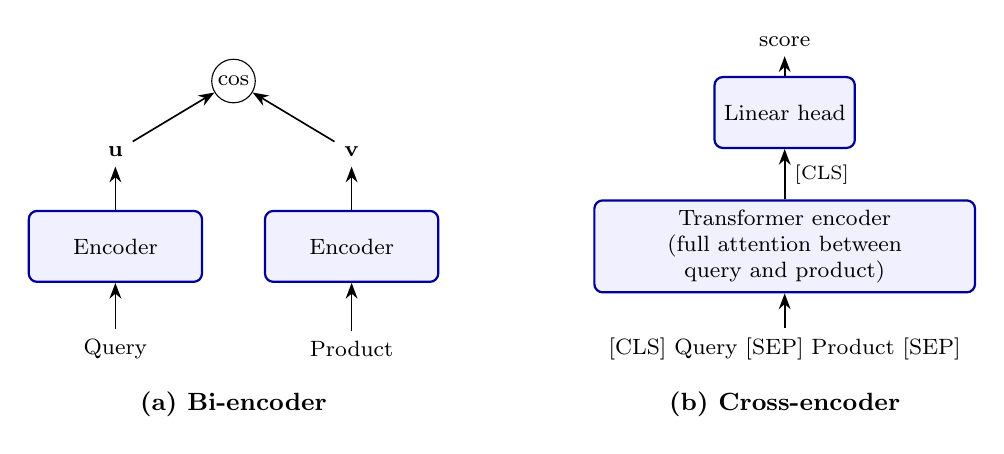
\begin{tikzpicture}[
  enc/.style={draw, rounded corners=3pt, fill=blue!6, draw=blue!60!black, thick, align=center, font=\footnotesize, minimum width=22mm, minimum height=9mm},
  txt/.style={align=center, font=\footnotesize},
  arr/.style={-{Stealth[length=2mm]}, semithick}]
  % bi-encoder
  \node[txt] (q1) at (0,0) {Query};
  \node[txt] (p1) at (3,0) {Product};
  \node[enc] (e1) at (0,1.3) {Encoder};
  \node[enc] (e2) at (3,1.3) {Encoder};
  \node[txt] (u) at (0,2.5) {$\mathbf{u}$};
  \node[txt] (v) at (3,2.5) {$\mathbf{v}$};
  \node[draw, circle, font=\footnotesize, inner sep=1.5pt] (cos) at (1.5,3.4) {$\cos$};
  \draw[arr] (q1) -- (e1); \draw[arr] (p1) -- (e2);
  \draw[arr] (e1) -- (u); \draw[arr] (e2) -- (v);
  \draw[arr] (u) -- (cos); \draw[arr] (v) -- (cos);
  \node[txt, font=\small\bfseries] at (1.5,-0.7) {(a) Bi-encoder};
  % cross-encoder
  \node[txt] (qp) at (8.5,0) {[CLS] Query [SEP] Product [SEP]};
  \node[enc, text width=46mm] (e3) at (8.5,1.3) {Transformer encoder\\(full attention between query and product)};
  \node[enc, minimum width=16mm] (head) at (8.5,3.0) {Linear head};
  \node[txt] (s) at (8.5,3.9) {score};
  \draw[arr] (qp) -- (e3); \draw[arr] (e3) -- node[right, font=\scriptsize]{[CLS]} (head); \draw[arr] (head) -- (s);
  \node[txt, font=\small\bfseries] at (8.5,-0.7) {(b) Cross-encoder};
\end{tikzpicture}
\caption{The two ways to match a query and a product with a pre-trained Transformer.}
\label{fig:encoders}
\end{figure}

\section{Transformer Backbones}
\textbf{MiniLM}~\cite{minilm} is a small Transformer (12 layers, hidden size 384) obtained by distilling the self-attention of a larger model. The MiniLM cross-encoder fine-tuned on the MS~MARCO passage ranking dataset is a popular, fast re-ranker and is the model of Amazon's baseline.

\textbf{DeBERTa-v3}~\cite{deberta} improves BERT in two ways. Its \emph{disentangled attention} represents each token by two vectors, one for content and one for relative position, and computes attention from content-to-content, content-to-position and position-to-content terms, which helps with word order. Version~3 is pre-trained with ELECTRA-style replaced-token detection, which is more sample-efficient than masked language modeling. DeBERTa-v3 was used by several top solutions of the competition. We use the base (184M parameters) and large (435M) sizes.

\section{Learning to Rank}
\label{sec:ndcg}
\textbf{Metric.} Ranking quality is measured by the normalized discounted cumulative gain~\cite{ndcg}:
\[
\mathrm{DCG}(q) = \sum_{i=1}^{|C_q|} \frac{g(y_{(i)})}{\log_2(i+1)},\qquad
\mathrm{nDCG}(q) = \frac{\mathrm{DCG}(q)}{\mathrm{IDCG}(q)},
\]
where $y_{(i)}$ is the label at rank $i$ and IDCG is the DCG of the ideal order. A relevant product near the top counts more than one further down, and the score is averaged over queries.

\textbf{Training objectives.} Learning-to-rank losses fall into three families. \emph{Pointwise} losses predict the relevance of each pair independently, by regression or classification. \emph{Pairwise} losses (e.g.\ RankNet) learn to order two products of the same query. \emph{Listwise} losses, such as ListNet~\cite{listnet}, compare the predicted distribution over the whole list with the target distribution.

\textbf{LambdaMART.} LambdaMART~\cite{lambdamart} trains gradient-boosted decision trees with gradients (``lambdas'') that weight each pair of products by the change in nDCG obtained by swapping them, so it optimizes the ranking metric directly. LightGBM~\cite{lightgbm} provides an efficient implementation (\texttt{lambdarank}) and is a standard way to combine heterogeneous features.

\textbf{Stacking.} When the score of one model is used as a feature of a second model, the second model must be trained on scores the first model produced for data it did not see. Otherwise the scores are over-confident on the training set and the second model learns to trust them too much. The usual solution is out-of-fold prediction: split the training data into $K$ folds, train $K$ models each without one fold, and score each fold with the model that did not see it~\cite{stacking}.

\section{The ESCI Challenge}\label{sec:esci}
The ESCI dataset~\cite{esci} was released with three tasks; Task~1 is the ranking of given candidates. Amazon's baseline fine-tunes the MiniLM cross-encoder on the query and the product title only and reports 0.857 nDCG on English. The top solutions reached about 0.90, averaged over three languages~\cite{top1,second,zhichun,practice}, so their scores are not directly comparable with an English-only result. They share a few ingredients: large DeBERTa-v3 cross-encoders that read more product fields; pointwise objectives (regression or 4-class classification), pairwise training being reported not to help~\cite{second}; techniques against noisy labels~\cite{top1,zhichun}; and, in one solution, a gradient-boosting stage over model outputs and list features~\cite{practice}. Large language models are not clearly better on this data~\cite{ebay}. Our system follows these ideas at a smaller scale and measures the effect of each.

% =====================================================================
\chapter{Dataset Analysis}\label{ch:data}
% =====================================================================
\section{Description}
We use the reduced version of the Shopping Queries Dataset (Apache-2.0), English part. It has 601,354 labeled query--product pairs for 29,844 queries, with an official train/test split (Table~\ref{tab:data}), and a catalog of 482,105 products with title, description, bullet points, brand and color. A third file gives the origin of each query (for example \texttt{negations} for queries built around a negation), which we use only for error analysis.

\textbf{Origin of the data.} The dataset was built by Amazon for the KDD Cup 2022~\cite{esci}. For each query, the candidate products are results returned by Amazon's search engine, and each query--product pair was labeled by human annotators as Exact, Substitute, Complement or Irrelevant. The product fields are the textual content of the product pages of the catalog. The data is distributed on GitHub (\texttt{amazon-science/esci-data}) under the Apache-2.0 license; we use it as released and do not collect additional data.

\begin{table}[H]
\centering
\caption{English portion of the reduced ESCI dataset.}
\label{tab:data}
\small
\begin{tabular}{@{}lrrcccc@{}}
\toprule
\textbf{Split} & \textbf{Queries} & \textbf{Pairs} & \textbf{E} & \textbf{S} & \textbf{C} & \textbf{I} \\
\midrule
Train & 20{,}888 & 419{,}653 & 43.3\% & 35.2\% & 4.5\% & 16.9\% \\
Test  & 8{,}956  & 181{,}701 & 43.9\% & 35.0\% & 4.5\% & 16.7\% \\
\bottomrule
\end{tabular}
\end{table}

\section{Main Observations}\label{sec:observations}
\begin{figure}[H]
\centering
\begin{minipage}[t]{0.49\linewidth}\centering
  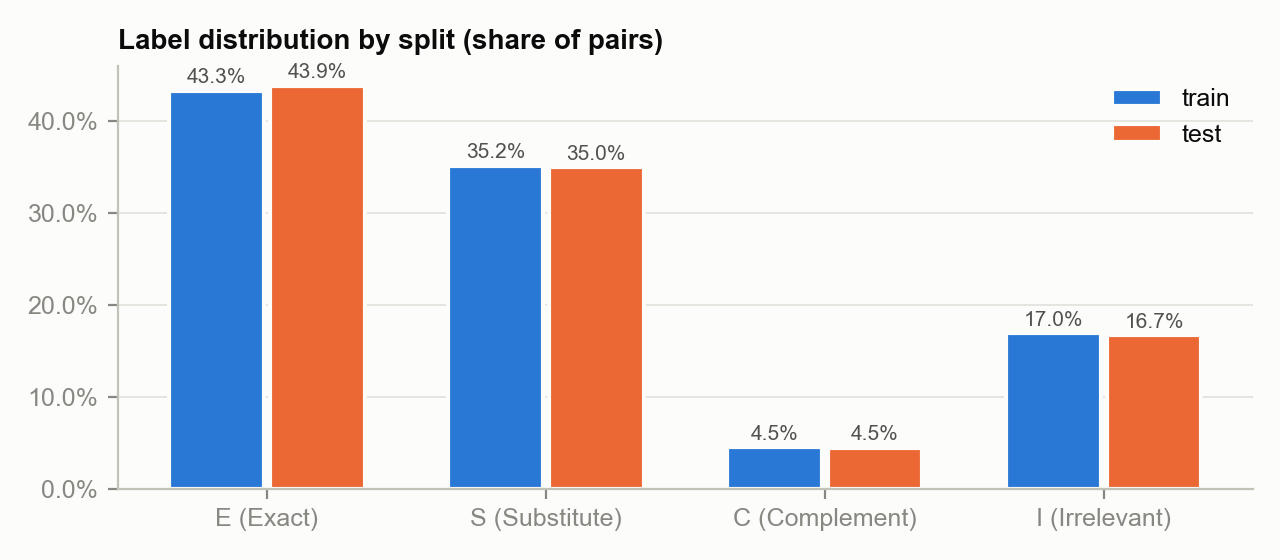
\includegraphics[width=\linewidth]{f1_label_share.png}\\[-2pt]{\small (a) label share}
\end{minipage}\hfill
\begin{minipage}[t]{0.49\linewidth}\centering
  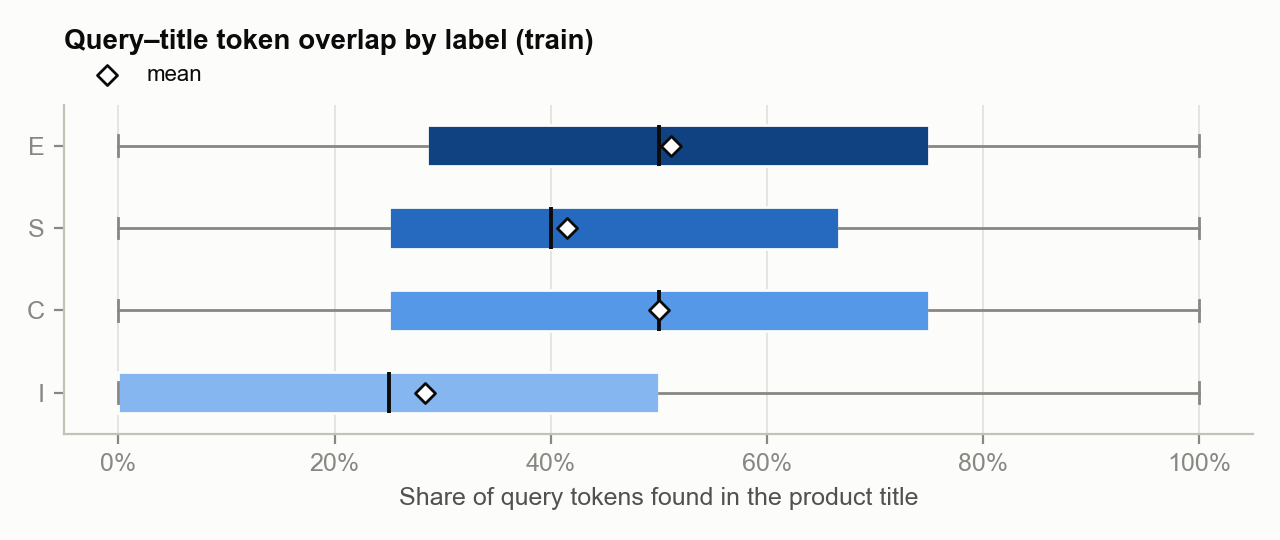
\includegraphics[width=\linewidth]{f6_overlap_by_label.png}\\[-2pt]{\small (b) query--title word overlap by label}
\end{minipage}\\[6pt]
\begin{minipage}[t]{0.49\linewidth}\centering
  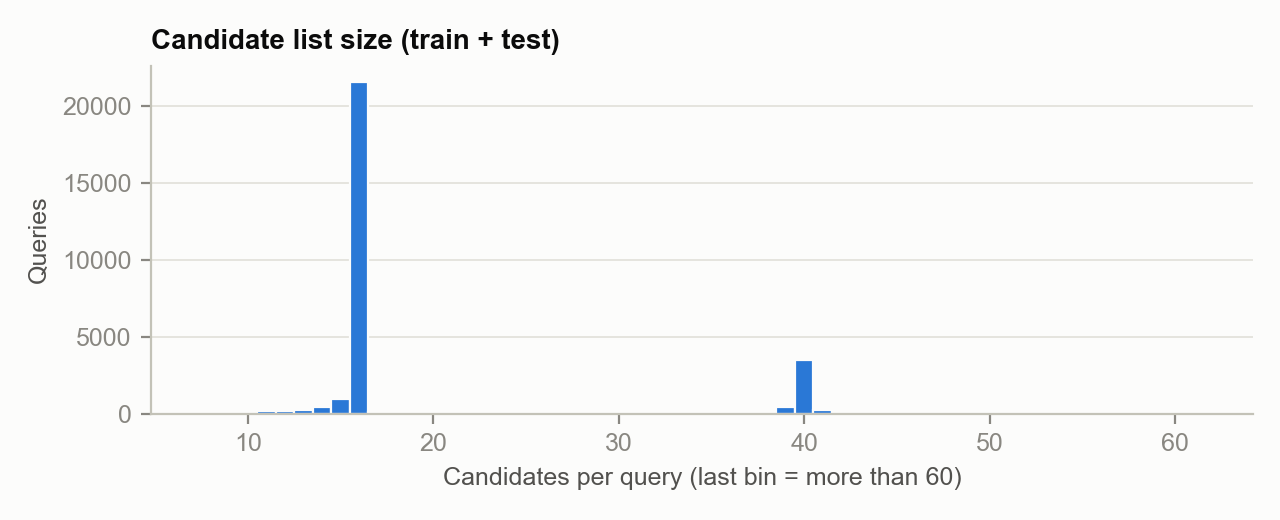
\includegraphics[width=\linewidth]{f2_candidates.png}\\[-2pt]{\small (c) candidates per query (train and test)}
\end{minipage}
\caption{Label distribution, word overlap and size of the candidate lists.}
\label{fig:eda}
\end{figure}

\paragraph{Candidate lists are short.} A query has 20.1 candidates on average, but the distribution has two peaks (Figure~\ref{fig:eda}c): 72\% of the queries have exactly 16 candidates and 14\% have between 39 and 41. 7.5\% have fewer than 16 (at least 8), and 1.4\% have more than 41 (at most 188). Because the lists are short, a model that reads every query--product pair jointly is affordable.

\paragraph{The hard part is Exact vs Substitute.} Exact and Substitute make up almost 80\% of the pairs (Figure~\ref{fig:eda}a) and 86\% of the queries have both. Since a Substitute is worth ten times less than an Exact product, the ranking depends mostly on putting Exact products above Substitutes, which often differ in a single attribute.

\paragraph{Shared words are a weak signal.} The share of query words found in the title separates Irrelevant products from the others, but barely separates Exact, Substitute and Complement (Figure~\ref{fig:eda}b). In 39\% of the (Exact, Substitute) pairs of a query, the overlap is exactly the same. A model must therefore understand attributes, not count words.

\paragraph{The metric has a narrow range.} A random order already reaches about 0.74 nDCG, and putting all Exact products first reaches 0.997. Differences between good systems are a few thousandths, so we compare systems with paired significance tests rather than single numbers.

\paragraph{Product text is incomplete.} The description is missing for 48\% of the products (and contains HTML for 29\%), the color for 32\%, the bullet points for 13\% and the brand for 6\%. The title is always present.

\paragraph{Labels are noisy.} Inside the same query, products with exactly the same title often get different labels (about one group in four). Some queries also have near-duplicates (``airpods case'', ``air pods case'') with the same candidates. Noise limits the score any model can reach; near-duplicates must be kept on the same side of a validation split.

\section{Preprocessing}
Cleaning is light: HTML entities are decoded, HTML tags removed, Unicode normalized and spaces collapsed. Case, numbers and units are kept because they carry the attributes that separate Exact from Substitute. The product text given to a model is one of three representations:
\begin{itemize}
  \item \texttt{title}: the title only, as in Amazon's baseline;
  \item \texttt{title\_bc}: \texttt{title [SEP] brand: X [SEP] color: Y};
  \item \texttt{main}: \texttt{title [SEP] brand: X [SEP] color: Y [SEP] bullet points}.
\end{itemize}
Missing fields are skipped. The description is not used: it is missing for half of the products, often repeats the bullet points and would not fit in the 256 tokens of the model.

\textbf{Validation set.} The official data has no validation set. We hold out 10\% of the training queries (2,089 queries, 41,513 pairs), splitting by groups of near-duplicate queries: 18,799 queries remain for training, no group is on both sides, and the label shares of the two parts differ by at most 0.94 percentage points. The official test split was not made by groups: 139 groups of near-duplicate queries have members in both train and test, and 155 test queries have a near-duplicate in the training set. We keep the official split for comparability with published results. All model choices are made on the validation set or by cross-validation on the training queries. The test set was scored three times; one decision, adding DeBERTa-v3-large to the final system, was taken after test scores had been seen (Section~\ref{sec:main}). The supplementary experiments are evaluated on validation only.

% =====================================================================
\chapter{System Design}\label{ch:method}
% =====================================================================
\section{Overview}
The system brings together ideas used by the top teams of the KDD Cup (Section~\ref{sec:esci}): a DeBERTa-v3 cross-encoder that reads several product fields, a pointwise training objective, and a gradient-boosting stage over model outputs and list features. Our aim is not a new method but a version of these ideas that fits a student compute budget, in which the effect of each component can be measured (Chapter~\ref{ch:exp}). Section~\ref{sec:reuse} lists which parts are reused and which were implemented in this project.

The system has two stages (Figure~\ref{fig:pipeline}). In the first stage, cross-encoders read the query together with a rich description of each product and estimate how likely the product is to be an exact match. In the second stage, a LightGBM model re-ranks each list using these estimates, how each candidate compares with the others in the same list, and simple lexical and semantic signals.

\begin{figure}[H]
\centering
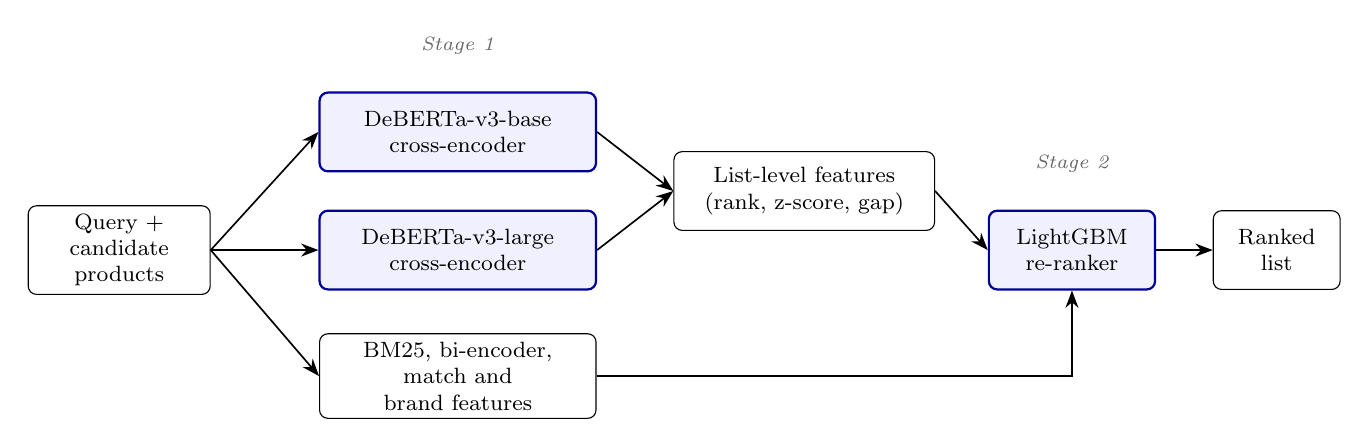
\begin{tikzpicture}[
  box/.style={draw, rounded corners=3pt, align=center, font=\footnotesize, minimum height=10mm, inner sep=3pt},
  acc/.style={box, draw=blue!60!black, fill=blue!6, thick},
  arr/.style={-{Stealth[length=2.2mm]}, semithick}]
  \node[box, text width=21mm]  (in)    at (0, 0)      {Query +\\candidate products};
  \node[acc, text width=33mm]  (base)  at (4.3, 1.5)  {DeBERTa-v3-base\\cross-encoder};
  \node[acc, text width=33mm]  (large) at (4.3, 0)    {DeBERTa-v3-large\\cross-encoder};
  \node[box, text width=33mm]  (feat)  at (4.3, -1.6) {BM25, bi-encoder,\\match and brand features};
  \node[box, text width=31mm]  (list)  at (8.7, 0.75) {List-level features\\(rank, z-score, gap)};
  \node[acc, text width=19mm]  (lgb)   at (12.1, 0)   {LightGBM\\re-ranker};
  \node[box, text width=14mm]  (out)   at (14.7, 0)   {Ranked\\list};
  \draw[arr] (in.east) -- (base.west);
  \draw[arr] (in.east) -- (large.west);
  \draw[arr] (in.east) -- (feat.west);
  \draw[arr] (base.east) -- (list.west);
  \draw[arr] (large.east) -- (list.west);
  \draw[arr] (list.east) -- (lgb.west);
  \draw[arr] (feat.east) -| (lgb.south);
  \draw[arr] (lgb) -- (out);
  \node[font=\scriptsize\itshape, text=black!60] at (4.3, 2.6) {Stage 1};
  \node[font=\scriptsize\itshape, text=black!60] at (12.1, 1.1) {Stage 2};
\end{tikzpicture}
\caption{The two-stage system. Shaded boxes are trained models.}
\label{fig:pipeline}
\end{figure}

Algorithm~1 summarizes the training and inference procedure.

\begin{center}
\fbox{\begin{minipage}{0.94\linewidth}
\small
\textbf{Algorithm 1.} Training and inference of the two-stage system.\\[-4pt]
\rule{\linewidth}{0.4pt}\\[2pt]
\textbf{Input:} training queries with labeled candidates; a query $q$ with candidates $C_q$ to rank.\\[2pt]
\textbf{Training}
\begin{enumerate}[leftmargin=*, itemsep=1pt, topsep=2pt]
  \item Clean the product fields and build the \texttt{main} text of every product.
  \item Split the training queries into five folds, keeping near-duplicate queries together.
  \item For each backbone $b \in \{$DeBERTa-v3-base, DeBERTa-v3-large$\}$ and each fold $k$: fine-tune a cross-encoder $M_{b,k}$ with the ce4 loss on the other four folds, and score fold $k$ with it (out-of-fold scores).
  \item Compute the BM25, bi-encoder, match, product and query features of every pair, and the list-context features of the cross-encoder scores within each query.
  \item Train the LightGBM \texttt{lambdarank} re-ranker on these features, with five-fold cross-validation on the same folds; keep the five fold models $R_1,\dots,R_5$.
\end{enumerate}
\textbf{Inference for a query $q$}
\begin{enumerate}[leftmargin=*, itemsep=1pt, topsep=2pt, resume]
  \item For each candidate $p \in C_q$, build the input \texttt{[CLS]} $q$ \texttt{[SEP]} text($p$) \texttt{[SEP]} and score it with every $M_{b,k}$; average the five scores and probabilities of each backbone.
  \item Compute the same features as in step 4 for all candidates of $q$.
  \item Score each candidate with the average of $R_1,\dots,R_5$ and sort $C_q$ by this score.
\end{enumerate}
\textbf{Output:} the ranked list of $C_q$.
\end{minipage}}
\end{center}

\section{Stage 1: Cross-Encoder Scorer}
\subsection{Input Representation}
Each pair is encoded as \texttt{[CLS]} query \texttt{[SEP]} product text \texttt{[SEP]} with the \texttt{main} representation (title, brand, color, bullet points). Brand, color and bullets contain most of the attributes that decide between Exact and Substitute, which the title alone often lacks. For example, for the test query \emph{``iphone 8 screen protector not plus''} one candidate is given to the model as:

\begin{center}
\begin{minipage}{0.92\linewidth}
\footnotesize\ttfamily\raggedright
[CLS] iphone 8 screen protector not plus [SEP] uShield Privacy Screen Protector for iPhone 8 Plus, iPhone 7 Plus - 3 Pack (w/Installation Frame) Tempered Glass Screen Protector Compatible with iPhone 8 Plus, 7 Plus (3 Pack)[Fit with Most Cases] [SEP] brand: uShield [SEP] Designed for Apple iPhone - Made for Apple iPhone 7+/8+. This new privacy screen protector will keep all your personal information away from the eyes of strangers around you. ; Everyday Protection - Features hydrophobic and oleophobic coating \ldots{} [SEP]
\end{minipage}
\end{center}

This product has no color, so the color field is skipped. When the sequence is longer than the limit, the tokenizer removes tokens from the end of the longer segment, which is almost always the product text, so the query and the beginning of the title are always kept.

\textbf{Sequence length.} With the \texttt{main} representation, the median product text has 95 words and 21\% of the texts are longer than about 190 words ($\approx$256 tokens). In a speed test before the full runs, one training epoch of DeBERTa-v3-base on a T4 was estimated at 1.6 hours with 192 tokens and 2.2 hours with 256 tokens. We chose 256 tokens, since the extra time keeps the bullet points of most products; the full run with 256 tokens took 2.4 hours.

\subsection{Model and Training}
We use DeBERTa-v3, in its base and large sizes, initialized from the public pre-trained weights. The classification head of Hugging Face Transformers takes the final hidden state of the \texttt{[CLS]} token, passes it through a dense layer and outputs one value (regression) or four values (classification).

The model is fine-tuned for one epoch on the 378,140 training pairs, in shuffled batches of 32 pairs (11,816 steps). The optimizer is AdamW with weight decay 0.01 (none on biases and layer normalization). The learning rate rises linearly during 1,200 warmup steps and then decreases linearly to zero; its peak is $2\cdot10^{-5}$ for the base model and $10^{-5}$ for the large model. Gradients are clipped to norm 1.0 and training uses mixed precision (fp16). There is no early stopping: the model after the last step is used.

\subsection{Training Objective}
The labels are ordered and the metric uses graded gains, so we considered three objectives. Let $s$ be the model output for a pair with label $y$:
\begin{itemize}
  \item \textbf{Regression (MSE)}, as in Amazon's baseline: one output trained with $\mathcal{L} = (s - g(y))^2$.
  \item \textbf{4-class classification (ce4)}: four outputs with softmax probabilities $p_E, p_S, p_C, p_I$, trained with cross-entropy on the label. The ranking score is the expected gain
  \[ s = p_E\,g(E) + p_S\,g(S) + p_C\,g(C) + p_I\,g(I). \]
  \item \textbf{Listwise (ListNet)}: one output; all candidates of a query are processed together, and the loss is the cross-entropy between the softmax of the scores in the list and the target distribution $t_i = g(y_i)/\sum_j g(y_j)$.
\end{itemize}
The final system uses ce4. It ranks as well as the others (Section~\ref{sec:loss}) and its class probabilities, in particular $p_E$, are useful features for the second stage.

\section{Out-of-Fold Training}
The second stage learns how much to trust the cross-encoder scores. If it were trained on scores that a cross-encoder produced for its own training pairs, these scores would be more confident and more accurate than on new queries, and the re-ranker would learn a weight that does not hold at test time. The training scores must therefore come from models that did not see the pairs they score.

We split the training queries into five folds of about 75,600 pairs, keeping near-duplicate queries in the same fold, and train five cross-encoders, each on four folds (about 302,500 pairs). Each fold is scored by the one model that did not see it, which gives an out-of-fold score for every training pair (Figure~\ref{fig:oof}). Validation and test pairs are scored by the average of the five models.

\begin{figure}[H]
\centering
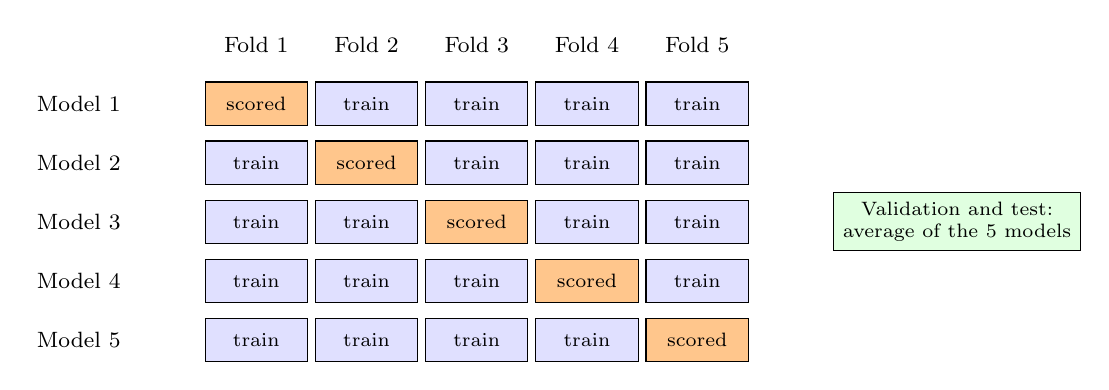
\begin{tikzpicture}[
  tr/.style={draw, fill=blue!12, minimum width=13mm, minimum height=5.5mm},
  ho/.style={draw, fill=orange!45, minimum width=13mm, minimum height=5.5mm},
  lab/.style={font=\footnotesize, anchor=east}]
  \foreach \m in {1,...,5} {
    \node[lab] at (-0.2, -0.75*\m) {Model \m};
    \foreach \f in {1,...,5} {
      \ifnum\f=\m \node[ho] at (1.4*\f, -0.75*\m) {\scriptsize scored};
      \else \node[tr] at (1.4*\f, -0.75*\m) {\scriptsize train}; \fi
    }
  }
  \foreach \f in {1,...,5} \node[font=\footnotesize] at (1.4*\f, 0) {Fold \f};
  \node[draw, fill=green!12, minimum width=27mm, minimum height=5.5mm, font=\scriptsize, align=center] at (10.3, -2.25) {Validation and test:\\average of the 5 models};
\end{tikzpicture}
\caption{Out-of-fold scoring. Each training pair is scored by the model trained without its fold.}
\label{fig:oof}
\end{figure}

Two checks show that the out-of-fold scores behave like the scores on unseen data. First, their spread on the training set is close to the spread on validation and test (standard deviation 0.286 against 0.279 for the base model). Second, each fold model trained on 80\% of the data scores between 0.8866 and 0.8888 on validation, against 0.8891 for the model trained on all training pairs: the smaller training set costs almost nothing. The average of the five fold models is even slightly more accurate than the single model (Section~\ref{sec:rerank}).

DeBERTa-v3-large does not fit a batch of 32 pairs of 256 tokens on one 16~GB T4 GPU. We train it with data parallelism on two T4 GPUs, each processing 16 pairs in four micro-batches with gradient accumulation, and mixed precision (fp16).

\section{Stage 2: Query-Context Re-Ranker}
A cross-encoder scores each pair alone. It cannot see that a product is the best of a weak list, that a score is high only because all candidates are similar, or that most of the list belongs to one brand. The second stage adds this context with 62 features in four families (Table~\ref{tab:features}).

\begin{table}[H]
\centering
\caption{Features of the re-ranker.}
\label{tab:features}
\small
\begin{tabularx}{\textwidth}{@{}l Y@{}}
\toprule
\textbf{Family} & \textbf{Features} \\
\midrule
Cross-encoder & Score and $p_E, p_S, p_C, p_I$ of the base and of the large model \\
List context & For these scores: rank, z-score and gap to the best candidate within the query; mean and standard deviation in the query; share of the list with the same brand, most frequent brand, number of brands \\
Lexical and semantic & BM25 on title and full text; share of query words in the title and text; number, unit and color match; brand mentioned in the query; negation check (``without X'' while the title contains X); bge and MiniLM bi-encoder similarities \\
Product and query & Text lengths and missing fields; query length; number of candidates; whether the query contains a number, unit, color or negation \\
\bottomrule
\end{tabularx}
\end{table}

\textbf{List-context features.} For a score $s$ of candidate $p$ in query $q$, the within-query features are its rank in the list, its z-score $z = (s - \mu_q)/\sigma_q$, where $\mu_q$ and $\sigma_q$ are the mean and standard deviation of the scores in the list, and its gap $s - \max_{p' \in C_q} s_{p'}$ to the best candidate. A decision tree splits a feature with one threshold for all queries. On raw scores, such a threshold means different things in different lists: in a list where every candidate scores high, a high score does not distinguish a product from its competitors. The z-score, rank and gap express the position of a candidate relative to the other candidates of the same query, which is what the ranking needs.

\textbf{LambdaMART objective.} The re-ranker is a LightGBM model with the \texttt{lambdarank} objective. For two candidates $i$ and $j$ of the same query with $i$ more relevant than $j$, LambdaMART uses the gradient
\[
\lambda_{ij} = \frac{-\sigma}{1 + e^{\sigma (s_i - s_j)}}\;\bigl|\Delta\mathrm{nDCG}_{ij}\bigr|,
\]
where $s_i, s_j$ are the current model scores and $|\Delta\mathrm{nDCG}_{ij}|$ is the change in nDCG if $i$ and $j$ were swapped~\cite{lambdamart}. Pairs whose swap would change the metric most receive the largest gradients. LightGBM expects integer relevance levels, so the labels are encoded as I~$=0$, C~$=1$, S~$=2$, E~$=3$. By default LightGBM would then use the gains $2^{l}-1 = (0, 1, 3, 7)$, which do not match the task. We therefore set the parameter \texttt{label\_gain} to $[0,\ 0.01,\ 0.1,\ 1]$, the official gains of levels 0 to 3, and evaluate nDCG over the full list, so that $\Delta\mathrm{nDCG}$ during training uses exactly the gains of the evaluation.

\textbf{Training.} The re-ranker is trained with five-fold cross-validation on the training queries, using the same folds as Stage~1. Each fold model stops when the nDCG of its held-out fold has not improved for 100 rounds, and validation and test lists are scored by the average of the five fold models. We use a learning rate of 0.05, 80\% of the features per tree and L2 regularization 1.0, and compared three tree sizes (15, 31 and 63 leaves, with at least 200, 100 and 50 pairs per leaf). The cross-validation nDCG of the three sizes differs by less than 0.001; the smallest is used, and its fold models stop after 112 to 345 rounds.

\section{Reused Components and Own Work}\label{sec:reuse}
\textbf{Reused.} The pre-trained models (MiniLM-L12 MS~MARCO cross-encoder, DeBERTa-v3-base and -large, the bge and MiniLM-L6 bi-encoders) are downloaded from Hugging Face. The settings of the baseline (model, input, loss, learning rate, warmup, one epoch) follow Amazon's public code. The overall design (rich product input, DeBERTa-v3, pointwise objectives, gradient boosting over model outputs) follows the published competition solutions. Model training uses the PyTorch, Hugging Face Transformers and LightGBM libraries.

\textbf{Implemented in this project.}
\begin{itemize}
  \item The evaluation module: nDCG over the full list with both gain mappings, nDCG@10, MRR, E-over-S, random tie-breaking and the paired bootstrap test.
  \item The data preparation: text cleaning, the three product representations, and the validation split and folds by groups of near-duplicate queries.
  \item The training loop of the cross-encoders with the three objectives, including the batching of whole candidate lists for ListNet.
  \item The training script for DeBERTa-v3-large on two GPUs (data parallelism with gradient accumulation).
  \item The out-of-fold pipeline, the 62 re-ranker features and the LightGBM training with cross-validation.
  \item The experiments, the significance tests and the error analysis.
\end{itemize}

% =====================================================================
\chapter{Experiments and Results}\label{ch:exp}
% =====================================================================
\section{Experimental Setup}
\textbf{Baselines.} (B1) BM25 on the \texttt{main} text, with inverse document frequencies over the whole catalog; (B2) the pre-trained bi-encoder bge-base-en-v1.5~\cite{bge}, without fine-tuning; (B3) our reproduction of Amazon's baseline: the MS~MARCO MiniLM cross-encoder fine-tuned on query and title with MSE.

\textbf{Metrics.} The main metric is nDCG over the full list with the official gains. We also report nDCG@10, the MRR of the first Exact product, and \emph{E-over-S}: the share of (Exact, Substitute) pairs of a query in which the Exact product is ranked higher. When two candidates have the same score, their order is chosen at random and the metric is averaged over three random orders.

\textbf{Gain mapping.} Amazon's public evaluation script swaps the gains of Substitute and Complement compared with the official definition of the challenge (Table~\ref{tab:gains}). Because Substitutes are much more frequent than Complements, the two mappings give different scores for the same ranking. All results in this report use the official mapping; the script's mapping is used only once, to check our reproduction of the published baseline (Section~\ref{sec:q1}).

\begin{table}[H]
\centering
\caption{The two gain mappings.}
\label{tab:gains}
\small
\begin{tabular}{@{}lcccc@{}}
\toprule
\textbf{Mapping} & \textbf{E} & \textbf{S} & \textbf{C} & \textbf{I} \\
\midrule
Official (challenge definition, used in this report) & 1 & 0.1 & 0.01 & 0 \\
Amazon's evaluation script & 1 & 0.01 & 0.1 & 0 \\
\bottomrule
\end{tabular}
\end{table}

\textbf{Significance.} Two systems are compared on the same test queries with a paired bootstrap on the per-query difference in nDCG (1,000 resamples)~\cite{bootstrap}; we call a difference significant when its 95\% confidence interval excludes zero. This interval covers the sampling of queries, not the randomness of training. To measure the latter, DeBERTa-v3-base (ce4) was trained with five seeds: their validation nDCG has a standard deviation of 0.0008 and a range of 0.0022 (0.8877--0.8899). Two seeds of MiniLM (\texttt{main} text, MSE) differ by 0.0031 on validation, with an interval that excludes zero. Differences below about 0.002 between single runs are therefore treated as ties, even when their interval excludes zero.

\textbf{Implementation and reproducibility.} All experiments ran in Kaggle notebooks, on one or two NVIDIA T4 GPUs (16~GB each) for the neural models and on CPU for LightGBM. Table~\ref{tab:env} lists the software versions (as recorded in the run logs; a few early baseline runs did not record them), models and seeds, and Table~\ref{tab:hparams} the main training settings.

\begin{table}[H]
\centering
\caption{Software, models, data and seeds.}
\label{tab:env}
\small
\begin{tabularx}{\textwidth}{@{}l Y@{}}
\toprule
\textbf{Item} & \textbf{Value} \\
\midrule
Software & Python 3.13, PyTorch 2.11 (CUDA 13.0 build), Transformers 5.20, LightGBM 4.6, pandas 2.3, NumPy 2.1 \\
Pre-trained models (Hugging Face) & \texttt{cross-encoder/ms-marco-MiniLM-L-12-v2}, \texttt{microsoft/deberta-v3-base}, \texttt{microsoft/deberta-v3-large}, \texttt{BAAI/bge-base-en-v1.5}, \texttt{sentence-transformers/all-MiniLM-L6-v2} \\
Data & Shopping Queries Dataset, \texttt{amazon-science/esci-data} on GitHub, reduced version, \texttt{us} locale \\
Seeds & 42 for every run and for the data split; 43 as a second seed for the MiniLM and DeBERTa-v3-base comparisons; 43--46 for the seed study of DeBERTa-v3-base (ce4) and 42--45 for the batching study (Section~\ref{sec:loss}) \\
\bottomrule
\end{tabularx}
\end{table}

\begin{table}[H]
\centering
\caption{Training settings (all cross-encoders: one epoch, batch 32, AdamW, linear schedule, fp16).}
\label{tab:hparams}
\small
\begin{tabular}{@{}lllrl@{}}
\toprule
\textbf{Model} & \textbf{Input} & \textbf{Learning rate} & \textbf{Max length} & \textbf{Training time} \\
\midrule
MiniLM-L12 (B3) & \texttt{title} & $7\cdot10^{-6}$ & 128 & 11 min, 1 T4 \\
DeBERTa-v3-base & \texttt{main} & $2\cdot10^{-5}$ & 256 & 2.4 h, 1 T4 \\
DeBERTa-v3-large & \texttt{main} & $1\cdot10^{-5}$ & 256 & 4.7 h, 2 T4 \\
LightGBM \texttt{lambdarank} & 62 features & 0.05 & -- & 2 min, CPU \\
\bottomrule
\end{tabular}
\end{table}

\section{Main Results}\label{sec:main}
Table~\ref{tab:main} compares the baselines, the intermediate models and the final system on the test set.

\begin{table}[H]
\centering
\caption{Main results: nDCG over the full list with the official gains on validation (2,089 queries) and test (8,956 queries), with the 95\% bootstrap confidence interval on test; secondary metrics on test. B3, MiniLM \texttt{main} and DeBERTa-v3-base: MSE loss, mean of two seeds (interval of seed 42). DeBERTa-v3-large: ce4 loss, average of the five fold models. $^{*}$LightGBM re-ranker on the base cross-encoder only, the final system before the large model was added (Section~\ref{sec:main}).}
\label{tab:main}
\small
\resizebox{\linewidth}{!}{%
\begin{tabular}{@{}llccccc@{}}
\toprule
 & \textbf{System} & \textbf{Val nDCG} & \textbf{Test nDCG [95\% CI]} & \textbf{nDCG@10} & \textbf{MRR} & \textbf{E-over-S} \\
\midrule
 & Random order & 0.742 & 0.746 [0.743, 0.749] & 0.576 & 0.609 & 0.500 \\
B1 & BM25 & 0.823 & 0.824 [0.821, 0.828] & 0.701 & 0.760 & 0.619 \\
B2 & bge bi-encoder (zero-shot) & 0.843 & 0.847 [0.844, 0.850] & 0.740 & 0.802 & 0.643 \\
B3 & MiniLM cross-encoder, title (Amazon) & 0.857 & 0.855 [0.852, 0.858] & 0.754 & 0.818 & 0.677 \\
\midrule
 & MiniLM cross-encoder, \texttt{main} & 0.868 & 0.866 [0.863, 0.869] & 0.772 & 0.835 & 0.695 \\
 & DeBERTa-v3-base, \texttt{main} & 0.888 & 0.887 [0.885, 0.890] & 0.809 & 0.866 & 0.730 \\
 & DeBERTa-v3-large, \texttt{main}, 5 folds & 0.897 & 0.897 [0.894, 0.899] & 0.824 & 0.880 & 0.744 \\
\midrule
 & First final system (base only, fixed before test)$^{*}$ & 0.895 & 0.892 [0.889, 0.895] & 0.817 & 0.874 & 0.733 \\
 & \textbf{Final system (two stages)} & \textbf{0.900} & \textbf{0.898 [0.895, 0.901]} & \textbf{0.827} & \textbf{0.882} & \textbf{0.745} \\
\bottomrule
\end{tabular}}
\end{table}

The final system reaches 0.898 nDCG, \textbf{+0.043 over Amazon's baseline} and +0.074 over BM25, and it improves all secondary metrics. In particular, it orders three out of four (Exact, Substitute) pairs correctly, against 62\% for BM25 and 68\% for the baseline. Against the baseline it improves 6,231 test queries and worsens 2,440. Our reproduction of the baseline (0.855, average of two seeds) is within 0.002 of the value reported in the ESCI paper (0.857), which confirms that our evaluation matches the official one. Validation and test scores agree closely, with differences below 0.004, so the choices made on validation carry over to the test set.

\textbf{How the final system was chosen.} The test set was scored three times, each time for every configuration evaluated so far.
(1) The first final system, a LightGBM re-ranker on the out-of-fold scores of the base cross-encoder, was fixed by cross-validation and validation before the first scoring; it reaches 0.892.
(2) The second scoring included the additional experiments, among them a single DeBERTa-v3-large model, whose test score (0.894) was therefore known when we decided to add the large model to the system.
(3) The large model was then trained on five folds and the re-ranker retrained on both cross-encoders. This version was accepted by a rule written before its run: it had to beat the weighted average of the large cross-encoder and the first re-ranker on cross-validation, with an interval above zero, and not be worse on validation (CV +0.0008 [0.0002, 0.0014], validation +0.0006). The test set was not used for this step.
The decision to try the large model is therefore the only one informed by the test set. Its effect, +0.0059 [0.0047, 0.0072] over the first final system, is much larger than the bias such a choice can introduce, but 0.898 should be read with this history in mind: 0.892 is the score of the system fixed before the test set was seen.

\section{Comparison of the Baselines (Q1)}\label{sec:q1}
Table~\ref{tab:baselines} gives all baseline variants on the \texttt{title} and \texttt{main} texts.

\begin{table}[H]
\centering
\caption{Baselines (nDCG on validation and test, E-over-S on test).}
\label{tab:baselines}
\small
\begin{tabular}{@{}llcccc@{}}
\toprule
\textbf{Model} & \textbf{Training on ESCI} & \textbf{Text} & \textbf{Val} & \textbf{Test} & \textbf{E-over-S} \\
\midrule
BM25 & no & \texttt{title} & 0.816 & 0.821 & 0.610 \\
BM25 & no & \texttt{main} & 0.823 & 0.824 & 0.619 \\
MiniLM-L6 bi-encoder & no & \texttt{title} & 0.820 & 0.828 & 0.606 \\
MiniLM-L6 bi-encoder & no & \texttt{main} & 0.826 & 0.831 & 0.614 \\
bge-base bi-encoder & no & \texttt{title} & 0.842 & 0.845 & 0.640 \\
bge-base bi-encoder & no & \texttt{main} & 0.843 & 0.847 & 0.643 \\
MiniLM-L12 cross-encoder (MS~MARCO) & no & \texttt{title} & 0.833 & 0.834 & 0.625 \\
MiniLM-L12 cross-encoder (B3) & yes & \texttt{title} & 0.857 & 0.855 & 0.677 \\
\bottomrule
\end{tabular}
\end{table}

\textbf{Dense models beat BM25, but not all of them by much.} On the same text, the small MiniLM-L6 bi-encoder is only 0.006--0.007 above BM25 on test, while bge-base is 0.023 above (significant on validation and test). The quality of the pre-trained encoder matters more than the dense approach itself. For both BM25 and the bi-encoders, adding brand, color and bullet points to the title helps only slightly (+0.002 to +0.004).

\textbf{Fine-tuning matters more than the architecture.} The MS~MARCO cross-encoder used without training on ESCI scores 0.834, below the bge bi-encoder, even though a cross-encoder can compare every query word with every product word. After fine-tuning on ESCI for one epoch it rises to 0.855 (+0.021). The notion of relevance in ESCI (``is this exactly the product I asked for?'') differs from the passage relevance of MS~MARCO, and the model has to learn it from the labels.

\textbf{Comparison with the published baseline.} Our B3 scores 0.8549 and 0.8555 with two random seeds, within 0.002 of the 0.857 reported in the ESCI paper. Amazon's evaluation script swaps the gains of Substitute and Complement; with that mapping our B3 scores 0.836, so the published value corresponds to the official gains used here. The paper also reports 0.675 for BM25. This value is lower than a random order of the candidates in our evaluation (0.746), so it must come from a different setup and is not used as a reference.

\section{Effect of Product Input and Backbone (Q2)}
Table~\ref{tab:d1} varies the product text and the backbone one at a time.

\begin{table}[H]
\centering
\caption{Test nDCG by product text and backbone (MSE loss; mean of two seeds where available).}
\label{tab:d1}
\small
\begin{tabular}{@{}lccc@{}}
\toprule
\textbf{Backbone} & \texttt{title} & \texttt{title\_bc} & \texttt{main} \\
\midrule
MiniLM-L12 (33M) & 0.855 & 0.858 & 0.866 \\
DeBERTa-v3-base (184M) & 0.877 & -- & 0.887 \\
DeBERTa-v3-large (435M)$^{*}$ & -- & -- & 0.894 \\
\bottomrule
\multicolumn{4}{@{}l}{\footnotesize $^{*}$ trained with the ce4 loss, one model.}
\end{tabular}
\end{table}

\begin{itemize}
  \item \textbf{Product text.} Adding brand and color helps a little (+0.003); adding the bullet points helps clearly (+0.010 for both MiniLM and DeBERTa, both significant). The bullet points contain the specifications (size, material, compatibility) that decide between Exact and Substitute.
  \item \textbf{Backbone.} Replacing MiniLM by DeBERTa-v3-base gives +0.021 on the same input, the largest single improvement of the project, and the large model adds another +0.007.
\end{itemize}
The two effects add up: going from MiniLM on titles to DeBERTa-v3-base on the full text is worth +0.032. The E-over-S score rises in the same way (0.677 $\rightarrow$ 0.730), showing that the gain comes from the hard Exact-versus-Substitute decisions.

\section{Effect of the Training Loss (Q3)}\label{sec:loss}
Table~\ref{tab:d2} compares the three training objectives with the model and data fixed.

\begin{table}[H]
\centering
\caption{nDCG of the three training objectives (MiniLM: mean of two seeds).}
\label{tab:d2}
\small
\begin{tabular}{@{}llccc@{}}
\toprule
\textbf{Model} & \textbf{Split} & \textbf{MSE} & \textbf{ce4} & \textbf{ListNet} \\
\midrule
MiniLM, \texttt{title} & validation & 0.857 & 0.857 & 0.858 \\
 & test & 0.855 & 0.856 & 0.858 \\
DeBERTa-v3-base, \texttt{main} & validation & 0.888 & 0.889 & -- \\
 & test & 0.887 & 0.887 & -- \\
\bottomrule
\end{tabular}
\end{table}

The differences are at most 0.003 and mostly not significant. ListNet is slightly better on test (+0.003) but not on validation, where one seed is better and one worse.

\textbf{Supplementary runs (validation only).} Three further experiments, run after the final system was fixed, refine this picture (Table~\ref{tab:losssupp}).
\begin{itemize}
  \item \textbf{A second seed for DeBERTa.} ce4 is ahead of MSE with both seeds (+0.0014 and +0.0022), +0.0018 [$-$0.0004, +0.0039] over the two: a small edge that is not significant.
  \item \textbf{MiniLM on the \texttt{main} text.} The order is reversed: ce4 is below MSE with both seeds, $-$0.0036 [$-$0.0060, $-$0.0010]. Which loss is better depends on the model.
  \item \textbf{Batching.} ListNet needs whole candidate lists in a batch, while MSE and ce4 were trained on shuffled pairs. To compare the losses on the same batches, MiniLM (\texttt{title}) was trained with all three losses on batches of whole queries, with four seeds. ListNet then beats MSE by +0.0036 [0.0014, 0.0057] with all four seeds, and ce4 is level with MSE. But batches of whole queries lower MSE by 0.0027 and ce4 by 0.0032 compared with shuffled pairs, while ListNet is unchanged. Most of ListNet's advantage in this setting therefore comes from the batching hurting the pointwise losses; against MSE trained on shuffled pairs it is about +0.001.
\end{itemize}

\begin{table}[H]
\centering
\caption{Supplementary loss comparisons on validation: paired difference $b - a$ in nDCG, per query averaged over seeds, with the 95\% bootstrap interval over the 2,089 queries. ``Same sign'': the difference has the same sign for every seed.}
\label{tab:losssupp}
\small
\resizebox{\linewidth}{!}{%
\begin{tabular}{@{}llcrc@{}}
\toprule
\textbf{Model, batches} & \textbf{$b - a$} & \textbf{Seeds} & \textbf{Difference [95\% CI]} & \textbf{Same sign} \\
\midrule
DeBERTa-v3-base, \texttt{main}, shuffled & ce4 $-$ MSE & 42, 43 & +0.0018 [$-$0.0004, +0.0039] & yes \\
MiniLM, \texttt{main}, shuffled & ce4 $-$ MSE & 42, 43 & $-$0.0036 [$-$0.0060, $-$0.0010] & yes \\
\midrule
MiniLM, \texttt{title}, whole queries & ListNet $-$ MSE & 42--45 & +0.0036 [+0.0014, +0.0057] & yes \\
MiniLM, \texttt{title}, whole queries & ce4 $-$ MSE & 42--45 & $-$0.0014 [$-$0.0037, +0.0013] & no \\
\midrule
MiniLM, \texttt{title}, MSE & whole queries $-$ shuffled & 42, 43 & $-$0.0027 [$-$0.0046, $-$0.0009] & yes \\
MiniLM, \texttt{title}, ce4 & whole queries $-$ shuffled & 42, 43 & $-$0.0032 [$-$0.0054, $-$0.0013] & yes \\
MiniLM, \texttt{title}, ListNet & whole queries $-$ shuffled & 42, 43 & $-$0.0002 [$-$0.0014, +0.0011] & no \\
\bottomrule
\end{tabular}}
\end{table}

\textbf{The training loss does not matter much for this task:} all differences stay below 0.004, close to the spread between two seeds of the same model (up to 0.003). With about 20 candidates per query, most of them Exact or Substitute, a good pointwise estimate of relevance is enough to order the list, which agrees with the experience of competition teams~\cite{second}. Training for a second epoch did not help either (0.886 vs 0.887 on test). We keep ce4 because it is at least as good as MSE on DeBERTa and its class probabilities are useful for the re-ranker.

\section{Effect of Query-Context Re-Ranking (Q4)}\label{sec:rerank}
Table~\ref{tab:d3} measures each part of the second stage on the test set.

\begin{table}[H]
\centering
\caption{Effect of the out-of-fold ensemble and of the re-ranker (test nDCG, paired difference with 95\% CI).}
\label{tab:d3}
\small
\begin{tabular}{@{}lcl@{}}
\toprule
\textbf{System} & \textbf{nDCG} & \textbf{Difference} \\
\midrule
DeBERTa-v3-large, one model on all training data & 0.894 & \\
DeBERTa-v3-large, average of 5 fold models & 0.897 & +0.003 [+0.002, +0.004] vs one model \\
Final: LightGBM re-ranker on base + large & 0.898 & +0.0015 [+0.0004, +0.0024] vs 5 folds \\
\midrule
\multicolumn{3}{@{}l}{\emph{With the base model only}} \\
DeBERTa-v3-base, average of 5 fold models & 0.889 & \\
LightGBM re-ranker on base & 0.892 & +0.003 [+0.002, +0.005] vs 5 folds \\
\bottomrule
\end{tabular}
\end{table}

\textbf{Ensembling the fold models} is better than one model trained on all data (+0.002 to +0.003), although each fold model sees only 80\% of the training data.

\textbf{The re-ranker} improves the ranking in both settings, but its gain shrinks as the cross-encoder gets stronger: +0.003 on top of the base model, +0.0015 on top of the large one. Much of what the list features add is already captured by a better cross-encoder. The gain remains significant, and the re-ranker is also the component that combines the two cross-encoders.

\textbf{Which features matter?} Table~\ref{tab:ablation} removes groups of features from the re-ranker. It is measured by cross-validation on the training queries and on validation, so that the test set is not used for this analysis.

\begin{table}[H]
\centering
\caption{Ablation of the re-ranker: nDCG and difference to the full model (paired bootstrap 95\% CI).}
\label{tab:ablation}
\small
\begin{tabular}{@{}lrccc@{}}
\toprule
\textbf{Features} & \textbf{Number} & \textbf{CV nDCG} & \textbf{CV difference} & \textbf{Val nDCG} \\
\midrule
All features & 62 & 0.8957 & -- & 0.8999 \\
Without the large cross-encoder & 48 & 0.8885 & $-0.0071$ [$-0.0081$, $-0.0063$] & 0.8943 \\
Without the base cross-encoder & 48 & 0.8947 & $-0.0010$ [$-0.0015$, $-0.0003$] & 0.8994 \\
Without the bi-encoder features & 55 & 0.8951 & $-0.0006$ [$-0.0011$, $-0.0001$] & 0.8989 \\
Without the lexical features & 50 & 0.8955 & $-0.0002$ [$-0.0006$, $+0.0002$] & 0.8992 \\
Cross-encoder features only & 28 & 0.8941 & $-0.0016$ [$-0.0022$, $-0.0010$] & 0.8980 \\
No cross-encoder feature & 34 & 0.8615 & $-0.0342$ [$-0.0358$, $-0.0327$] & 0.8607 \\
\bottomrule
\end{tabular}
\end{table}

The large cross-encoder carries most of the information: without it the re-ranker loses 0.007. Each other family is worth 0.001 or less on its own, but together the non-cross-encoder features are worth 0.0016, a significant amount. Without any cross-encoder feature the re-ranker still reaches 0.861 on validation, above the fine-tuned MiniLM baseline (0.857): lexical, bi-encoder and list features together are worth a small fine-tuned cross-encoder.

Table~\ref{tab:importance} lists the features that the trees use most, measured by the total gain of the splits on each feature. The two most important are the within-query z-scores of the large model's score and of its $p_E$, which together account for about 70\% of the gain. The re-ranker relies mostly on how a candidate compares with the rest of its list, which is the information the cross-encoder alone does not have.

\begin{table}[H]
\centering
\caption{The five most important features of the final re-ranker (share of the total split gain).}
\label{tab:importance}
\small
\begin{tabular}{@{}llr@{}}
\toprule
\textbf{Feature} & \textbf{Description} & \textbf{Share} \\
\midrule
large score, z-score & z-score of the large model's expected gain within the query & 51.0\% \\
large $p_E$, z-score & z-score of the large model's $p_E$ within the query & 18.4\% \\
base score, z-score & z-score of the base model's expected gain within the query & 6.8\% \\
large score, gap & difference to the best large-model score in the query & 3.9\% \\
base score, rank & rank of the base model's score within the query & 2.2\% \\
\bottomrule
\end{tabular}
\end{table}

\section{Error Analysis (Q5)}\label{sec:errors}
\paragraph{By query source.} The dataset records how each query was collected. Table~\ref{tab:source} gives the test nDCG of the main systems for each source. Queries of the \texttt{negations} source, built around a negation, are the hardest for every system. They are also where training helps most: from BM25 to the final system the score rises by 0.100, against 0.075 for the \texttt{other} source. On these queries the re-ranker adds nothing over the large cross-encoder (0.851 for both). The \texttt{nlqec} source has only 30 queries, too few to draw conclusions.

\begin{table}[H]
\centering
\caption{Test nDCG by query source.}
\label{tab:source}
\small
\begin{tabular}{@{}lrccccc@{}}
\toprule
\textbf{Source} & \textbf{Queries} & \textbf{BM25} & \textbf{bge} & \textbf{B3} & \textbf{Large, 5 folds} & \textbf{Final} \\
\midrule
other & 7,233 & 0.828 & 0.853 & 0.856 & 0.901 & 0.903 \\
parse\_pattern & 781 & 0.849 & 0.863 & 0.873 & 0.895 & 0.895 \\
negations & 689 & 0.751 & 0.760 & 0.821 & 0.851 & 0.851 \\
behavioral & 223 & 0.852 & 0.865 & 0.865 & 0.891 & 0.893 \\
nlqec & 30 & 0.723 & 0.838 & 0.768 & 0.888 & 0.875 \\
\bottomrule
\end{tabular}
\end{table}

\paragraph{Two negation queries.} Table~\ref{tab:negexamples} shows the top three products of BM25 and of the final system for two test queries of the \texttt{negations} source. BM25 rewards the negated word: for \emph{``laptop not chromebook''} its top products are Chromebooks and a Chromebook keyboard, and for \emph{``iphone 8 screen protector not plus''} they are protectors for the iPhone 8 Plus, all labeled Irrelevant or Substitute. The final system puts the Exact products first. Its nDCG on these two queries is 1.000 and 0.997, against 0.400 and 0.441 for BM25. The MiniLM baseline (B3), which reads only the title, already reaches 0.996 and 0.940. These examples therefore show the benefit of a fine-tuned cross-encoder over BM25 on negations; on them the title-only baseline is already nearly correct.

\begin{table}[H]
\centering
\caption{Top three products for two negation queries (test set), with their labels.}
\label{tab:negexamples}
\footnotesize
\begin{tabularx}{\textwidth}{@{}c Y c Y c@{}}
\toprule
\textbf{Rank} & \textbf{BM25} & & \textbf{Final system} & \\
\midrule
\multicolumn{5}{@{}l}{\emph{Query: ``laptop not chromebook''}} \\
1 & Keyboard replacement for HP ChromeBook 11 G5 & I & HP Stream 11.6-inch HD laptop, Windows 10 Home & E \\
2 & Lenovo Chromebook C330 2-in-1 convertible laptop & I & HP Stream 14-inch laptop, Windows 10 Home & E \\
3 & ASUS Chromebook C200MA 11.6" laptop & I & ASUS VivoBook L203MA ultra-thin laptop & E \\
\midrule
\multicolumn{5}{@{}l}{\emph{Query: ``iphone 8 screen protector not plus''}} \\
1 & OMOTON tempered glass protector for iPhone 8 Plus / 7 Plus & S & Ailun screen protector for iPhone 8, 7, 6s, 6 (4.7-inch) & E \\
2 & JETech screen protector for iPhone 8 Plus and 7 Plus & I & Tech Armor film protector for iPhone SE 2020, 7, 8 (4.7-inch) & E \\
3 & Purity glass screen protector for iPhone 8 Plus / 7 Plus & I & amFilm screen protector for iPhone SE (2020), 8, 7, 6S, 6 & E \\
\bottomrule
\end{tabularx}
\end{table}

\paragraph{By query type.} Figure~\ref{fig:property} groups the test queries by simple properties. The final system improves over the baseline in every group (by +0.03 to +0.05, all significant). The hardest queries are those containing a \textbf{negation} (0.853 vs 0.902 for the others), followed by long queries (six words or more) and queries with numbers. For numbers, a random order is also lower (0.715 vs 0.754), so part of the gap comes from harder candidate lists. Queries that mention the brand of a candidate are the easiest (0.913).

\begin{figure}[H]
\centering
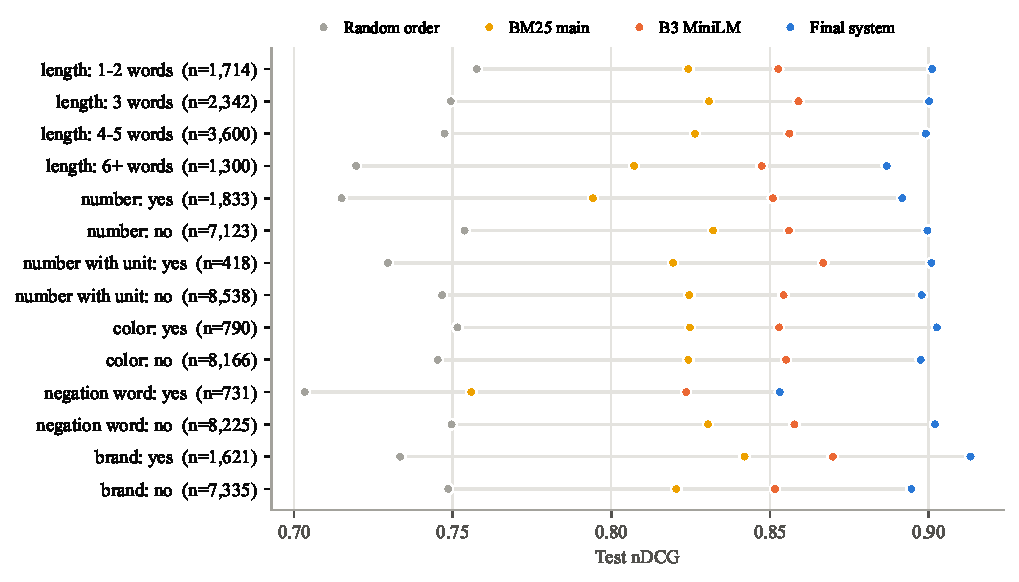
\includegraphics[width=0.92\linewidth]{fig_query_property.pdf}
\caption{Test nDCG by query property. The random order shows how hard each group of lists is before any model.}
\label{fig:property}
\end{figure}

\paragraph{Do the models read the negation?} Negation queries are the hardest group, and the one where the re-ranker adds nothing over the large cross-encoder (Table~\ref{tab:source}). Two explanations are possible: the models ignore the negated phrase, or the labels do not penalize products that contain the excluded item. We tested both on validation (supplementary experiment). Of the 186 validation queries with a negation cue, we kept by hand the 129 that ask for a product X without Y, removing book titles, slogans and product names such as ``no show socks''. Each query was scored in four versions: as written (``X without Y''), without the negated phrase (``X''), with the exclusion turned into an inclusion (``X with Y''), and with another cue (``X no Y''). A product is tagged \emph{has} when its title or bullet points mention Y, and \emph{negated} when they state its absence (``no Y'', ``Y-free''). Table~\ref{tab:negprobe} reports, for each model: the share of \emph{has} products scored lower for ``X without Y'' than for ``X with Y'' (0.5 means that the model ignores the negation), the share of \emph{negated} products scored higher, the Kendall $\tau$ between the rankings for ``without'' and ``no'', and the nDCG of the query as written minus that of the query without the negated phrase, with the real labels. DeBERTa-v3-large and the final system could not be probed because their weights were not kept.

\begin{table}[H]
\centering
\caption{Negation probe on 129 validation queries (ranges over seeds). \emph{Has} lower: share of products that contain Y scored lower when Y is excluded (114 queries with such products). \emph{Negated} higher: share of products that state ``no Y'' scored higher (67 queries). $\tau$: agreement of the rankings for ``without'' and ``no''. $\Delta$nDCG: nDCG of the query as written minus that of the query without the negated phrase.}
\label{tab:negprobe}
\small
\resizebox{\linewidth}{!}{%
\begin{tabular}{@{}llcccc@{}}
\toprule
\textbf{Model (\texttt{main} text)} & \textbf{Seeds} & \textbf{\emph{Has} lower} & \textbf{\emph{Negated} higher} & \textbf{$\tau$} & \textbf{$\Delta$nDCG} \\
\midrule
MiniLM, ce4 & 42, 43 & 0.87--0.88 & 0.71 & 0.80--0.81 & +0.043 to +0.055 \\
MiniLM, distilled ($\alpha = 0$ and $0.5$) & 42, 43 & 0.82--0.84 & 0.80--0.89 & 0.81--0.84 & +0.051 to +0.057 \\
DeBERTa-v3-base, ce4 & 43--46 & 0.72--0.78 & 0.92--0.96 & 0.88--0.90 & +0.054 to +0.071 \\
\bottomrule
\end{tabular}}
\end{table}

All models react to the negation: every share is well above 0.5, with intervals over queries that exclude it, and keeping the negated phrase improves nDCG under the real labels by 0.04 to 0.07, so the labels do reward reading it. The models differ in how they read it. MiniLM lowers almost every product that mentions Y, including products that say they do not contain it; DeBERTa-v3-base separates the two cases and gives more similar rankings for ``without'' and ``no''. The \emph{has} tag is a string match and also catches mentions such as ``compatible with Y'', so its share is not expected to reach 1. The distilled MiniLMs (Section~\ref{sec:discussion}) move toward the behavior of their DeBERTa teacher. For models of base size, the probe therefore rules out the two simplest explanations: the models do not ignore the negation, and the labels are not indifferent to it. Why this group stays the hardest, and why the re-ranker does not help on it, remains open.

\paragraph{Where labels end up.} Figure~\ref{fig:labelpos} shows the average position of each label in the ranked lists. The distance between Exact and Substitute products doubles from BM25 (0.10) to the final system (0.20), most of it coming from the DeBERTa backbone. Complements, which BM25 ranks close to Exact products because they share the product name (``case for iPhone 12''), are pushed down to the level of Irrelevant products by the trained models.

\begin{figure}[H]
\centering
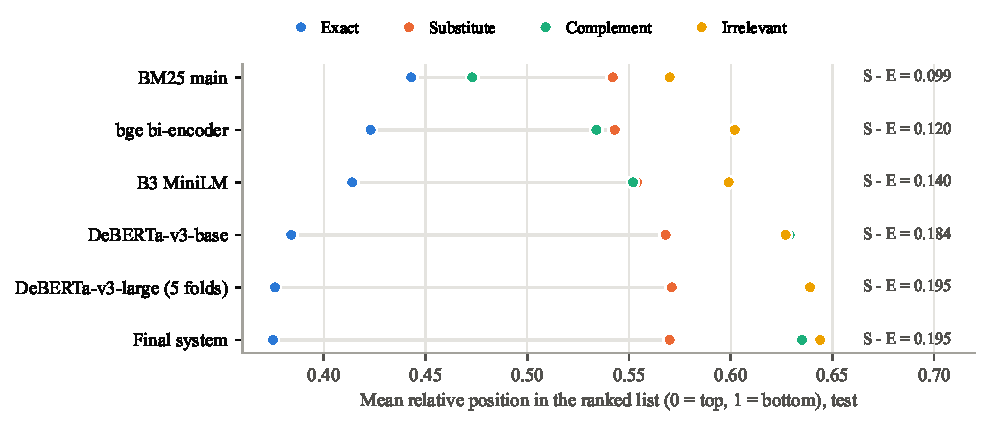
\includegraphics[width=0.92\linewidth]{fig_label_position.pdf}
\caption{Average relative position of each label in the ranked list (0 = top, 1 = bottom), test set.}
\label{fig:labelpos}
\end{figure}

\paragraph{Gains and losses per query.} Compared with the baseline B3, the final system improves 6,231 of the 8,956 test queries and worsens 2,440; the others are unchanged. 1,758 queries gain more than 0.1 nDCG and 447 lose more than 0.1. The large losses are concentrated on lists with few Exact products: among the 50 queries with the largest loss, 56\% have one or two Exact products, against 14\% of all test queries. When a list has a single Exact product, moving it from the first to the second position alone can cost about a third of the score.

\paragraph{Worst queries.} Table~\ref{tab:worst} lists four of the queries with the lowest nDCG. In each case the only product labeled Exact is clearly not what the query asks for, and the system ranks it near the bottom, which is arguably correct. Other failures come from input problems, such as an HTML entity left in the query or a query made of a product code.

\begin{table}[H]
\centering
\caption{Examples among the worst test queries: the single Exact product and its rank in the final system.}
\label{tab:worst}
\small
\begin{tabularx}{\textwidth}{@{}p{5cm} c Y@{}}
\toprule
\textbf{Query} & \textbf{Rank of E} & \textbf{Product labeled Exact} \\
\midrule
``tortillas without interesterified soybean oil'' & 37 / 39 & Fish oil 1000 mg softgels \\
``fake weed jar'' & 15 / 16 & Dried catnip buds (cat treats) \\
``cryptid'' & 11 / 16 & A product titled ``The Awakening'' \\
``airport face mask kids'' & 11 / 15 & Inflatable neck pillow \\
\bottomrule
\end{tabularx}
\end{table}

\paragraph{Summary.} Remaining errors come from three sources: constraints in the query that must be checked against product attributes (negations, numbers, long specifications); lists with a single Exact product, where one swap costs much of the score; and noisy labels, which cap the score any model can reach.

\section{Discussion}\label{sec:discussion}
\paragraph{Gain versus cost.} Table~\ref{tab:cost} puts the main steps next to their training cost. The largest gains are also the cheapest: moving from MiniLM on titles to DeBERTa-v3-base on the full product text adds 0.032 for 2.4 hours of training on one GPU. The large model adds 0.007 for about four times the GPU time (4.7 hours on two GPUs, against 2.4 hours on one). The last steps, five-fold training of both models and the re-ranker, add another 0.004 but need about 35 hours of training (about 59 GPU-hours). Returns therefore diminish quickly, and in a setting with limited compute or strict latency, DeBERTa-v3-base on the \texttt{main} text alone would keep most of the improvement.

We nevertheless keep the second stage in the final system for two reasons. It is the component that combines the two cross-encoders with the list context, and it gave the best cross-validation and validation scores, the criteria used for all choices (CV +0.0008 [0.0002, 0.0014] over the simple weighted average of the large cross-encoder and a base-model re-ranker). On test it is significantly better than the large cross-encoder alone (+0.0015), but not than that weighted average (+0.0005). Scoring the 223,214 validation and test pairs takes 22 minutes with the base model on one T4 and 30 minutes with the large model on two T4.

\begin{table}[H]
\centering
\caption{Test nDCG and training cost of the main steps (T4 GPUs on Kaggle).}
\label{tab:cost}
\small
\begin{tabular}{@{}lcl@{}}
\toprule
\textbf{System} & \textbf{Test nDCG} & \textbf{Training cost} \\
\midrule
MiniLM cross-encoder, \texttt{title} (B3) & 0.855 & 11 min, 1 GPU \\
MiniLM cross-encoder, \texttt{main} & 0.866 & 34 min, 1 GPU \\
DeBERTa-v3-base, \texttt{main} & 0.887 & 2.4 h, 1 GPU \\
DeBERTa-v3-large, \texttt{main} & 0.894 & 4.7 h, 2 GPUs \\
DeBERTa-v3-large, 5 fold models & 0.897 & 23.4 h, 2 GPUs \\
Final system (two stages) & 0.898 & + about 12 h, 1 GPU (base folds) \\
\bottomrule
\end{tabular}
\end{table}

\paragraph{Can the large model be distilled into a small one?} As a supplementary experiment (validation only, two seeds), MiniLM on the \texttt{main} text was trained on the out-of-fold class probabilities of the five large models~\cite{kd}, alone ($\alpha = 0$) or mixed half and half with the labels ($\alpha = 0.5$). The distilled model clearly beats a MiniLM trained with ce4 on the labels (+0.0063 [0.0042, 0.0082], same sign for both seeds), but ce4 is the weaker loss for MiniLM (Section~\ref{sec:loss}). Against MSE, the best MiniLM, the gain is +0.0027 [$-$0.0001, +0.0057] (+0.0039 and +0.0015 for the two seeds), about the difference between two MSE seeds (0.0031). With teacher probabilities only, the distilled MiniLM reaches 0.871 on validation against 0.897 for the teacher: it recovers about 10\% of the gap. Its probabilities are also less calibrated (expected calibration error 0.04, against 0.025 for ce4). At this scale, distillation is not a cheap substitute for the large model.

\paragraph{Relation to the competition solutions.} Our results are consistent with the choices of the top teams described in Section~\ref{sec:esci}. A strong DeBERTa-v3 encoder that reads more product fields gives the largest improvement; a pointwise objective is sufficient, since neither classification nor a listwise loss clearly beats regression; and a gradient-boosting stage over model outputs and list features gives a smaller but consistent gain. Our final score cannot be compared directly with the leaderboard, which averages three languages.

\paragraph{What the results suggest.} Two observations go beyond the comparison of numbers. First, the cross-encoder used without training on ESCI was weaker than a bi-encoder, and became the best baseline only after fine-tuning: the task's definition of relevance has to be learned from its labels. Second, the analysis of the worst queries shows that some failures are labeling problems, so further improvements of the model will be increasingly hard to measure on this test set.

% =====================================================================
\chapter{Conclusion}\label{ch:conclusion}
% =====================================================================
\section{Summary}
We built a two-stage ranking system for Task~1 of the ESCI challenge: DeBERTa-v3 cross-encoders reading a rich product description, followed by a LightGBM re-ranker with list-level features. It reaches 0.898 test nDCG on the English data, +0.043 over Amazon's cross-encoder baseline; the version fixed before the test set was first used reaches 0.892 (Section~\ref{sec:main}). The experiments answer the five questions as follows:
\begin{enumerate}[label=\textbf{Q\arabic*}]
  \item Fine-tuned cross-encoders beat bi-encoders, which beat BM25; fine-tuning on the task matters more than the architecture.
  \item What the model reads and how large it is matter most: the bullet points add +0.010 and DeBERTa-v3 adds +0.021 over MiniLM (+0.007 more for the large size).
  \item The training loss matters little: regression, classification and listwise losses are within 0.004, the best one depends on the model, and the advantage of the listwise loss comes mostly from how batches are formed.
  \item Re-ranking with list context adds a small but significant gain, which shrinks as the cross-encoder gets stronger.
  \item The system is weakest on queries with negations, long specifications and numbers, and on lists with a single Exact product; some of the worst queries have doubtful labels. Models of base size do react to negations and the labels reward it, so the cause of the weakness on negation queries remains open.
\end{enumerate}

\section{Practical Implications}
For an e-commerce search engine, the results suggest three points. First, the product attributes that sellers already provide (brand, color, bullet points) are worth giving to the ranking model: they improve the ranking at no extra data cost. Second, a cross-encoder must score every candidate of every query, so its cost grows with the number of candidates. In our runs, scoring the 223,214 validation and test pairs took 22 minutes for DeBERTa-v3-base on one T4 GPU (about 170 pairs per second) and 30 minutes for DeBERTa-v3-large on two T4 GPUs (about 120 pairs per second). This is acceptable for re-ranking a short list of 16--40 candidates, but not for scoring a whole catalog, where a fast first stage such as BM25 or a bi-encoder remains necessary. Third, since most of the gain comes from the base model with rich input, the large model and the second stage are worth their cost only where small improvements in ranking quality matter. Distilling the large model into MiniLM recovered only about a tenth of the gap between them in our runs, so a fast model still costs ranking quality.

\section{Limitations}
\begin{itemize}
  \item The test set was scored three times, and the decision to add DeBERTa-v3-large to the final system was taken after its test score was known. The system fixed before any test scoring reaches 0.892; 0.898 is the score after this decision (Section~\ref{sec:main}). No untouched held-out set remains.
  \item Most cross-encoders were trained with a single seed. Five seeds of DeBERTa-v3-base give a validation standard deviation of 0.0008 (range 0.0022), and two MiniLM seeds differ by 0.0031, so differences of about 0.002 between single runs are within seed variation. The seed variance of the LightGBM re-ranker was not measured.
  \item On test, the final re-ranker is not significantly better than a simple weighted average of the large cross-encoder and a re-ranker built on the base cross-encoder.
  \item The negation probe covers only DeBERTa-v3-base and MiniLM, because the weights of DeBERTa-v3-large and of the final system were not kept, and 129 validation queries; test queries were not added, so as not to score the test set again. The labels of negation queries were not audited by hand.
  \item The supplementary experiments (Sections~\ref{sec:loss}, \ref{sec:errors} and~\ref{sec:discussion}) are measured on validation only.
  \item Only the English, reduced data was used, and labels were taken as given.
  \item Compute limited the largest model to DeBERTa-v3-large trained for one epoch.
\end{itemize}

\section{Future Work}
\begin{itemize}
  \item Training that is robust to label noise, such as label smoothing or removing pairs flagged by confident learning~\cite{cleanlab}.
  \item Adding a cross-encoder from a different model family (e.g.\ bge-reranker) as a third score: in a preliminary experiment, averaging it with DeBERTa improved the ranking although it is weaker alone.
  \item Dedicated handling of negations and numbers, the weakest query types.
  \item Extending to the other languages and to full-catalog retrieval, with a bi-encoder retrieving the candidates that the cross-encoder then re-ranks.
\end{itemize}

% =====================================================================
\renewcommand{\bibname}{References}
\begin{thebibliography}{99}\small
\addcontentsline{toc}{chapter}{References}
\bibitem{esci} C.~K. Reddy, L.~M\`arquez, F.~Valero, N.~Rao, H.~Zaragoza, S.~Bandyopadhyay, A.~Biswas, A.~Xing, K.~Subbian. \emph{Shopping Queries Dataset: A Large-Scale ESCI Benchmark for Improving Product Search}. arXiv:2206.06588, 2022.
\bibitem{aicrowd} AIcrowd. \emph{ESCI Challenge for Improving Product Search}. \url{https://www.aicrowd.com/challenges/esci-challenge-for-improving-product-search}
\bibitem{top1} Q.~Zhang, Z.~Yang, Y.~Huang, Z.~Chen, Z.~Cai, K.~Wang, J.~Zheng, J.~He, J.~Gao. \emph{A Semantic Alignment System for Multilingual Query-Product Retrieval}. arXiv:2208.02958, 2022.
\bibitem{second} X.~Qin, N.~Liang, H.~Zhang, W.~Zou, W.~Zhang. \emph{Second Place Solution of Amazon KDD Cup 2022: ESCI Challenge for Improving Product Search}. KDD Cup 2022 Workshop.
\bibitem{zhichun} X.~Cui, W.~Xiong, S.~Wang. \emph{ZhichunRoad at Amazon KDD Cup 2022: MultiTask Pre-Training for E-Commerce Product Search}. KDD Cup 2022 Workshop.
\bibitem{practice} F.~Wu, Y.~Liu, R.~Gazo, B.~Bedrich, X.~Qu. \emph{Some Practice for Improving the Search Results of E-commerce}. KDD Cup 2022 Workshop.
\bibitem{ebay} C.~Palen-Michel, R.~Wang, Y.~Zhang, D.~Yu, C.~Xu, Z.~Wu. \emph{Investigating LLM Applications in E-Commerce}. arXiv:2408.12779, 2024.
\bibitem{tfidf} G.~Salton, C.~Buckley. \emph{Term-Weighting Approaches in Automatic Text Retrieval}. Information Processing \& Management 24(5), 1988.
\bibitem{bm25} S.~Robertson, H.~Zaragoza. \emph{The Probabilistic Relevance Framework: BM25 and Beyond}. Foundations and Trends in Information Retrieval 3(4), 2009.
\bibitem{sbert} N.~Reimers, I.~Gurevych. \emph{Sentence-BERT: Sentence Embeddings using Siamese BERT-Networks}. EMNLP-IJCNLP 2019.
\bibitem{bge} S.~Xiao, Z.~Liu, P.~Zhang, N.~Muennighoff. \emph{C-Pack: Packaged Resources To Advance General Chinese Embedding}. arXiv:2309.07597, 2023.
\bibitem{monobert} R.~Nogueira, K.~Cho. \emph{Passage Re-ranking with BERT}. arXiv:1901.04085, 2019.
\bibitem{minilm} W.~Wang, F.~Wei, L.~Dong, H.~Bao, N.~Yang, M.~Zhou. \emph{MiniLM: Deep Self-Attention Distillation for Task-Agnostic Compression of Pre-Trained Transformers}. NeurIPS 2020.
\bibitem{deberta} P.~He, J.~Gao, W.~Chen. \emph{DeBERTaV3: Improving DeBERTa using ELECTRA-Style Pre-Training with Gradient-Disentangled Embedding Sharing}. arXiv:2111.09543, 2021.
\bibitem{listnet} Z.~Cao, T.~Qin, T.-Y.~Liu, M.-F.~Tsai, H.~Li. \emph{Learning to Rank: From Pairwise Approach to Listwise Approach}. ICML 2007.
\bibitem{lambdamart} C.~J.~C. Burges. \emph{From RankNet to LambdaRank to LambdaMART: An Overview}. Microsoft Research Technical Report MSR-TR-2010-82, 2010.
\bibitem{lightgbm} G.~Ke, Q.~Meng, T.~Finley, T.~Wang, W.~Chen, W.~Ma, Q.~Ye, T.-Y.~Liu. \emph{LightGBM: A Highly Efficient Gradient Boosting Decision Tree}. NeurIPS 2017.
\bibitem{stacking} D.~H. Wolpert. \emph{Stacked Generalization}. Neural Networks 5(2), 1992.
\bibitem{ndcg} K.~J\"arvelin, J.~Kek\"al\"ainen. \emph{Cumulated Gain-Based Evaluation of IR Techniques}. ACM Transactions on Information Systems 20(4), 2002.
\bibitem{bootstrap} B.~Efron, R.~J. Tibshirani. \emph{An Introduction to the Bootstrap}. Chapman \& Hall, 1993.
\bibitem{cleanlab} C.~G. Northcutt, L.~Jiang, I.~L. Chuang. \emph{Confident Learning: Estimating Uncertainty in Dataset Labels}. JAIR 70, 2021.
\bibitem{kd} G.~Hinton, O.~Vinyals, J.~Dean. \emph{Distilling the Knowledge in a Neural Network}. arXiv:1503.02531, 2015.
\end{thebibliography}

\end{document}
